\documentclass[]{beamer}
% Class options include: notes, notesonly, handout, trans,
%                        hidesubsections, shadesubsections,
%                        inrow, blue, red, grey, brown

% Theme for beamer presentation.
%\usepackage{beamerthemesplit} 
% Other themes include: beamerthemebars, beamerthemelined, 
%                       beamerthemetree, beamerthemetreebars  

\usepackage{graphicx}

\title{Population management in the face of evolution}    
\author{Shaun Coutts, Robert Freckelton, Helen Hicks, Dylan Childs}                
\institute{University of Sheffield, UK}      % Enter your institute name between curly braces
%\date{\today}                    % Enter the date or \today between curly braces

\begin{document}

% Creates title page of slide show using above information
\begin{frame}
  \titlepage
\end{frame}

\section{Herbicide is great}
\begin{frame}
	\frametitle{Herbicide is great}
	\begin{columns}[c]
		\column{2.4in}
		more weeds $\Rightarrow$ less crops
		\\~\\
		hand weeding fields estimated \\ at 60hr / ha \\(http://www.ncfar.org/\\
		ncfar\_africa.pdf)
		\\~\\
		crop rotations and fallow periods

		\column{2.5in}
		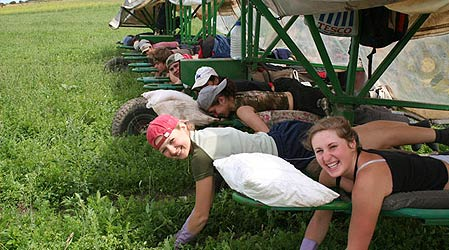
\includegraphics[width=2.3in]{hand_weeding}	
	\end{columns}	
\end{frame}

\begin{frame}
	\frametitle{Black grass (\textit{Alopecurus myosuroides})}
	\begin{columns}[c]	
		\column{2.5in}
			\includegraphics[width=2.5in]{field_work_BG}
	
		\column{2.5in}	
			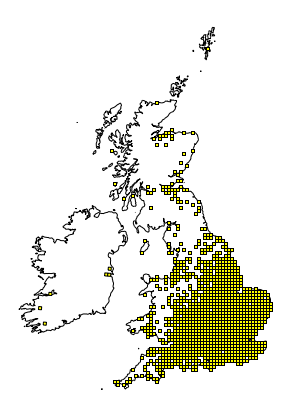
\includegraphics[width=2.2in]{BG_map.png}
			\\~
			https://data.nbn.org.uk
	\end{columns} 
\end{frame}

\begin{frame}
	\includegraphics[width=4in]{BG_photo_herb_app}
\end{frame}

\section{modelling herbicide resistance}
\begin{frame}
	\frametitle{herbicide resistance}
	\begin{center}
		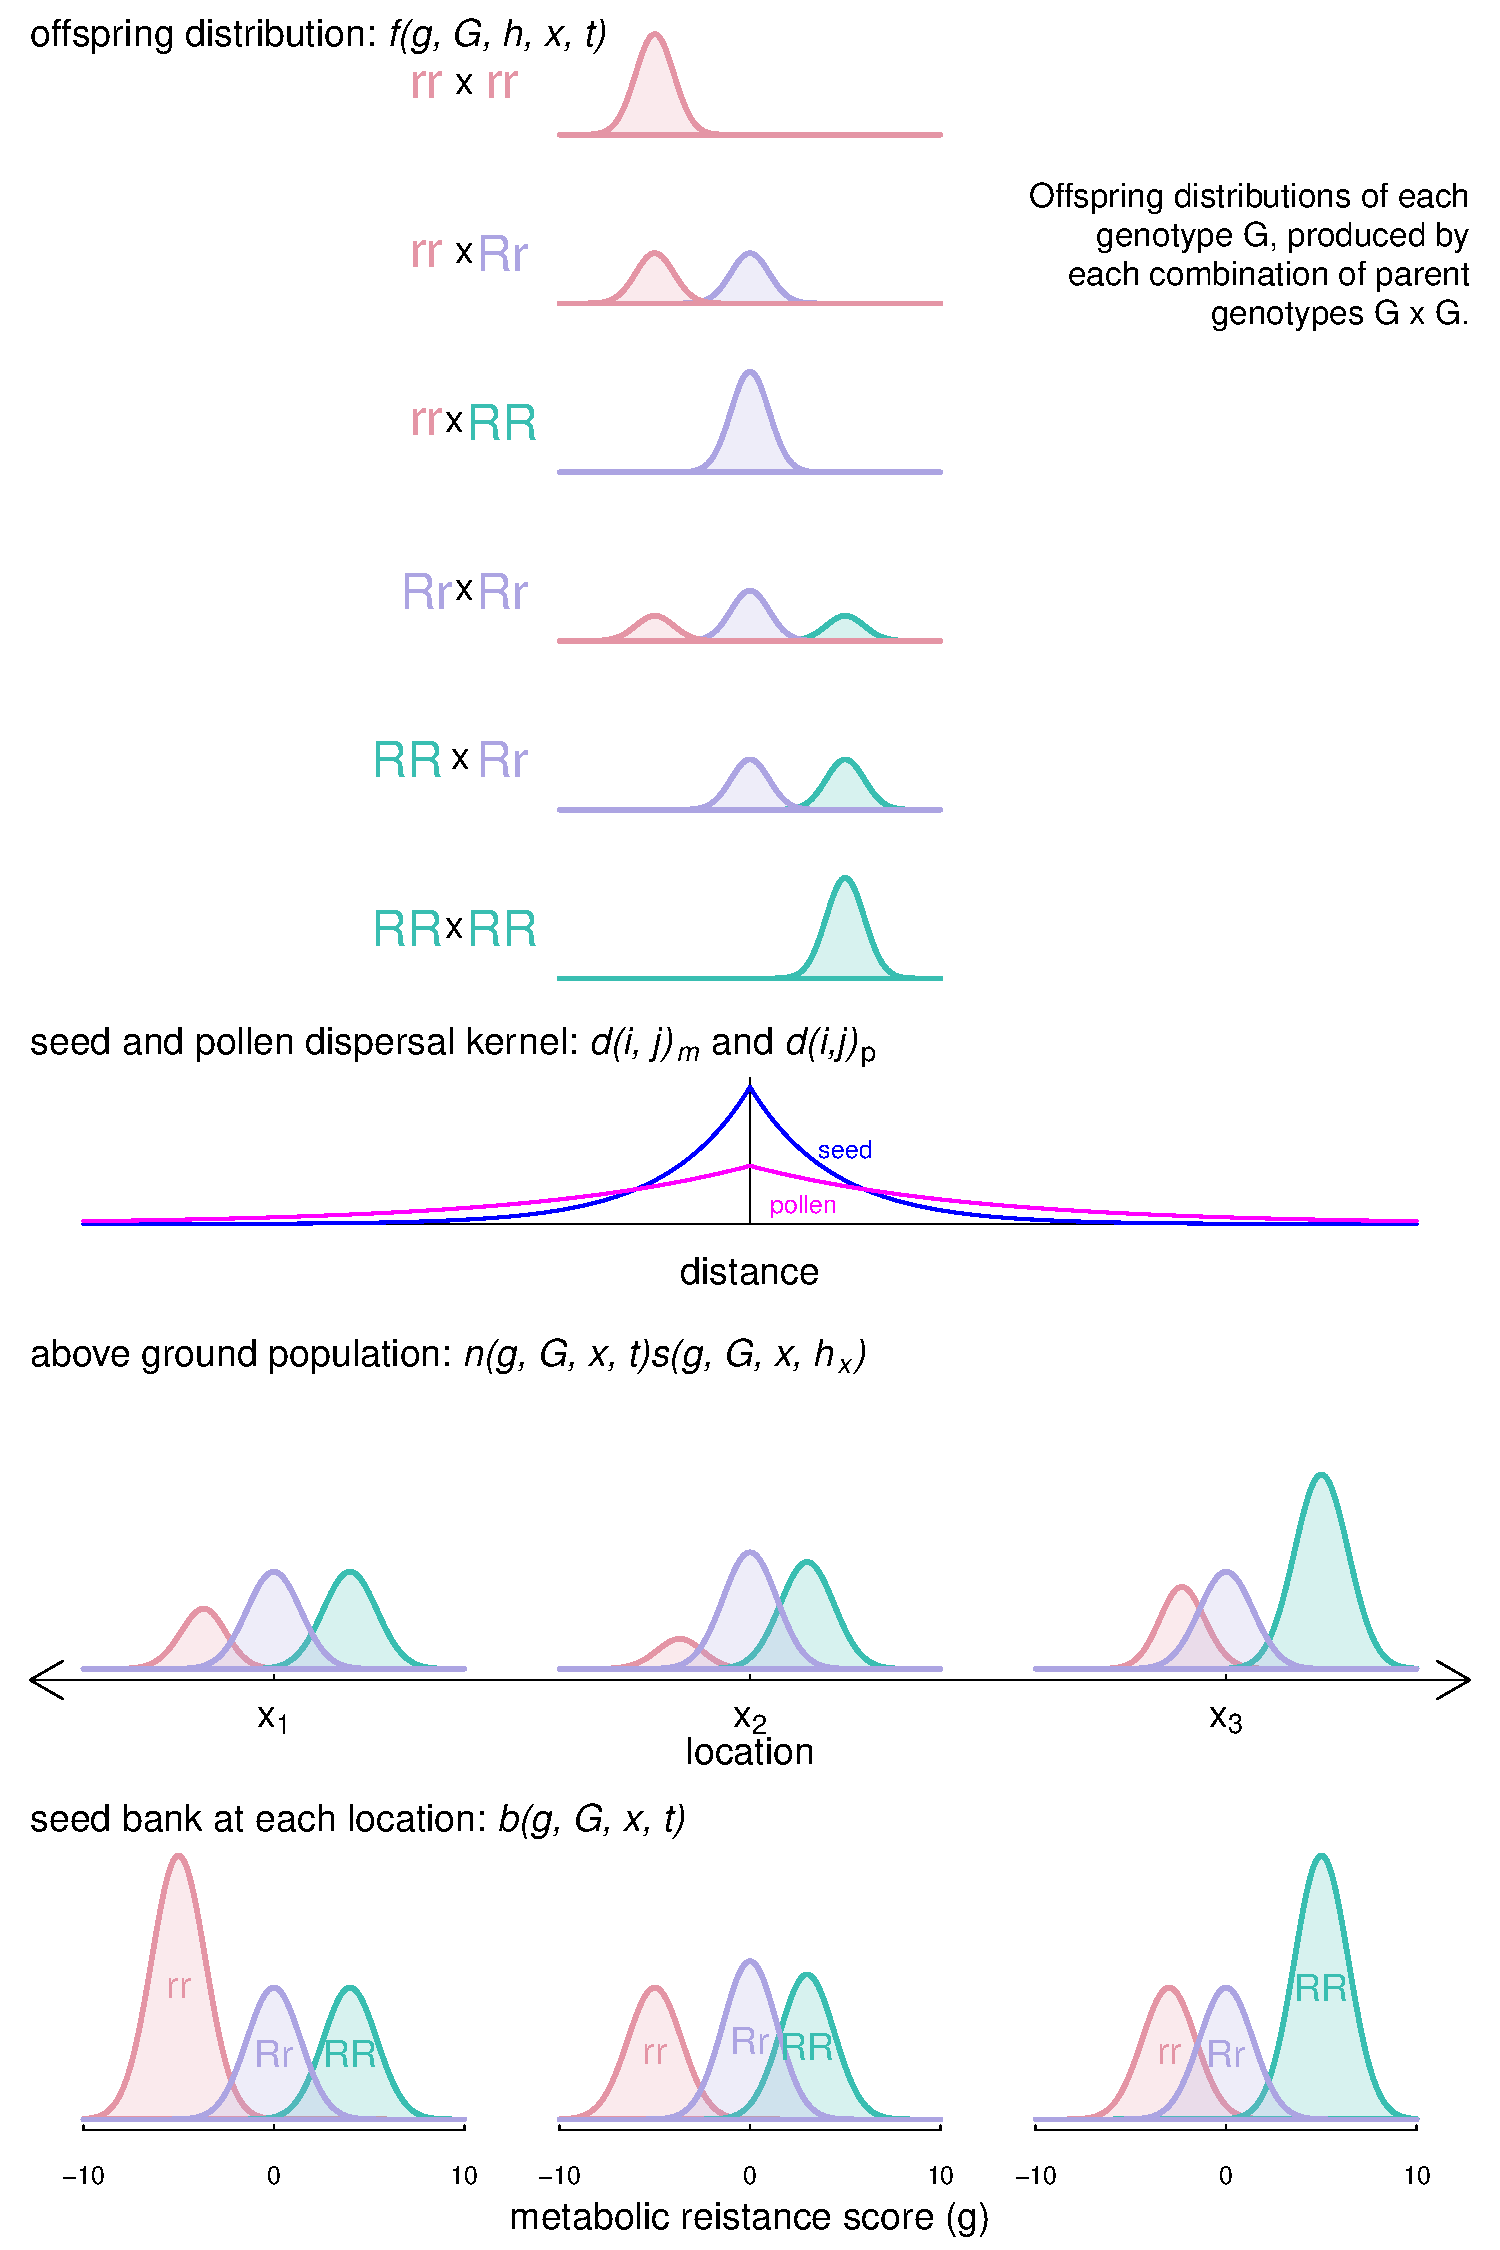
\includegraphics[width=2.2in]{BG_pop_spatial_mod_schematic.pdf}\\
	\end{center} 
\end{frame}

\begin{frame}
	\frametitle{If there are two ways to be resistant, why use both?}
	\begin{center}
		\includegraphics[width=3.0in]{space_time_blank.png} 
	\end{center}
\end{frame}

\begin{frame}
	\frametitle{If there are two ways to be resistant, why use both?}
	\begin{center}
		\includegraphics[width=3.0in]{inv_full_ls.png} 
	\end{center}
\end{frame}

\begin{frame}
	\frametitle{If there are two ways to be resistant, why use both?}
	\begin{center}
		\includegraphics[width=3.0in]{inv_empty_ls.png} 
	\end{center}
\end{frame}

\section{what to do about it}
\begin{frame}
	\frametitle{Integrated weed management}
	 \begin{columns}[c] %slides 3in by 5in and I have 
	 \column{2.5in}
	 	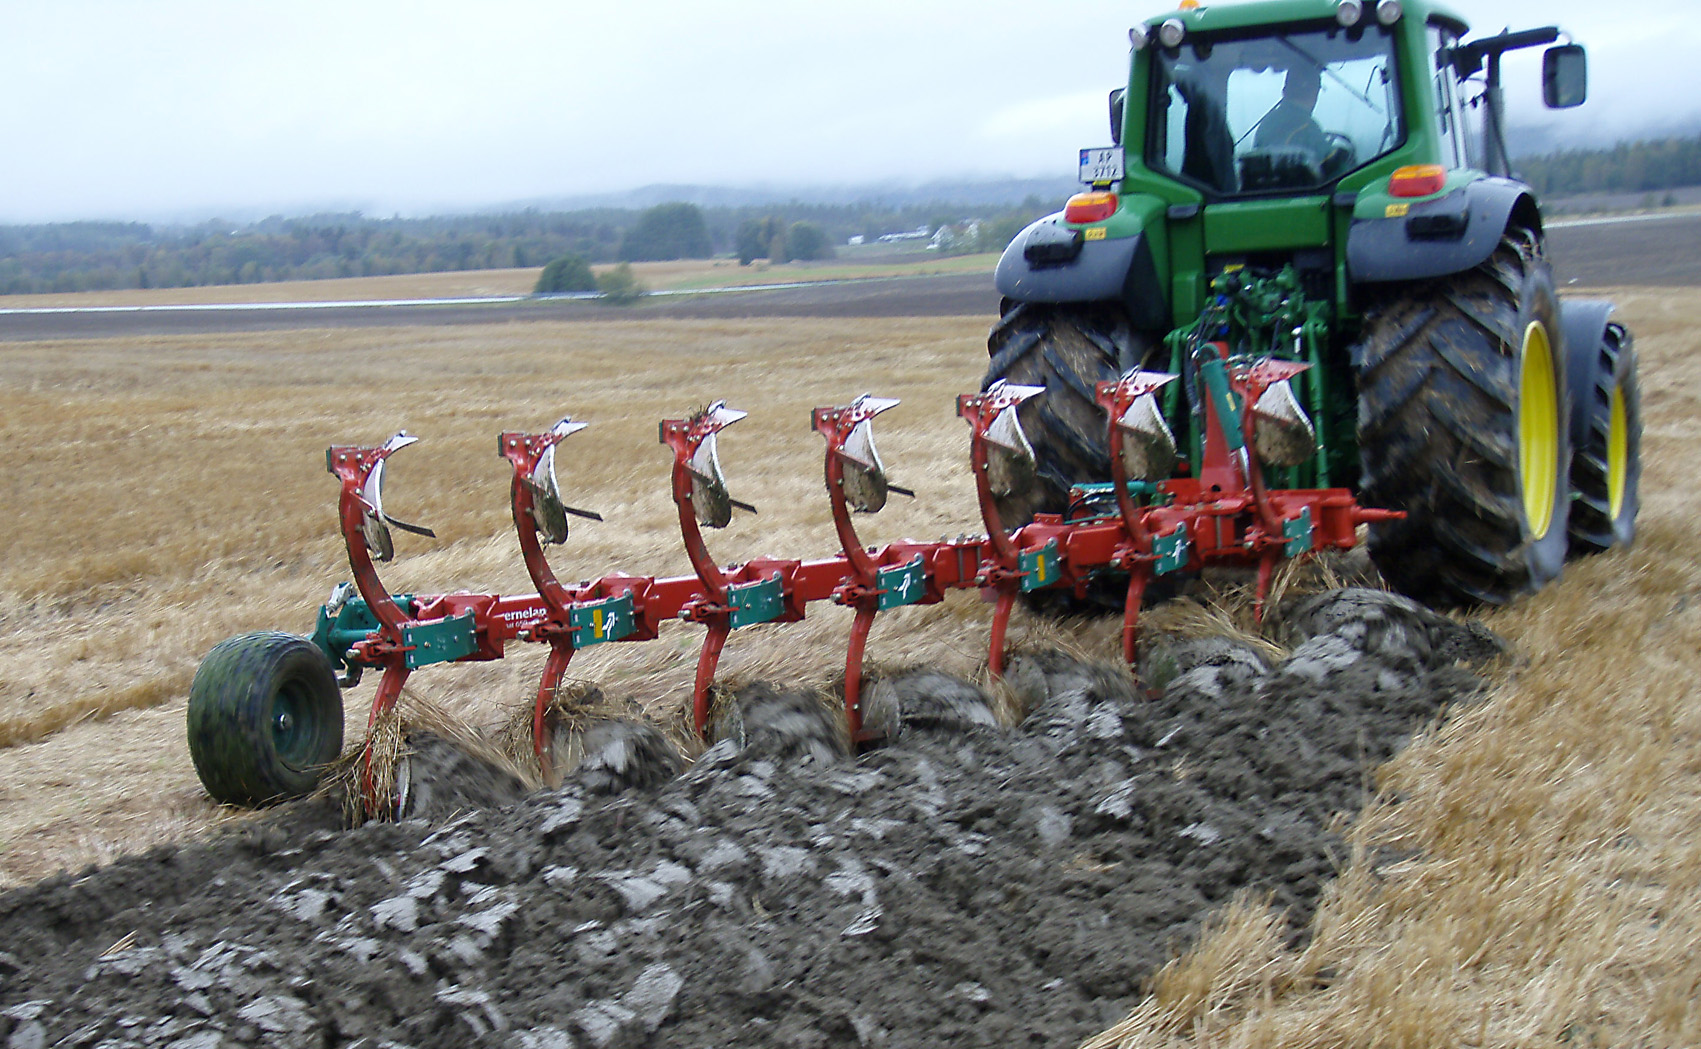
\includegraphics[width=1.5in]{Plowing_ecomat}
	 	\\~\\
	 	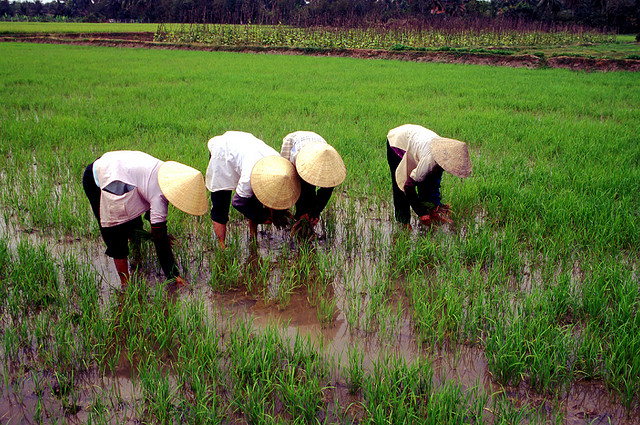
\includegraphics[width=1.5in]{weeds-manual-hand}	
	 \column{2.5in}
	 	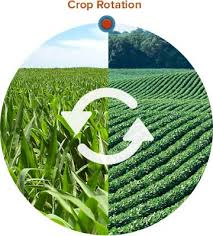
\includegraphics[width=1.5in]{crop-rotation}
	 \end{columns}
\end{frame}

\section{IWM as combinatorial optimisation}  
  \begin{frame}
    \frametitle{Integrated weed management as a combinatorial optimization problem}
    Five management options:
    \begin{itemize}
      \item \textbf{Crop choice:} winter wheat, alternative, fallow
      \item \textbf{Direct action:} herbicide, mechanical control, plowing to remove seeds from seed bank, planting wheat at high density to reduce black grass fecundity.  
    \end{itemize}       
    ~\\
    There are 25 different set of these management options which make logical sense.
    \\~\\
    each set is one action, e.g. \{wheat, herbicide, no mechanical control, no plowing, standard planting density\}  
  \end{frame}
  
  \begin{frame}
    \frametitle{Integrated weed management as a combinatorial optimization problem}
    If $T = 20$ years there are number of actions$^T$ possible actions sequences 
    \\~\\
    Very BIG number\\
    $25^{20} = 9.094947 \times 10^{27}$ 
  \end{frame}

  \begin{frame}
    \frametitle{Integrated weed management as a combinatorial optimization problem}
     The goal is to find the sequence of actions over a given time horizon, $T$, that maximizes an objective function 
     \\~\\
    Objective function: maximize discounted economic returns.
    \\~\\
    Other objective functions are possible that include a wider range of goals, such as social stigma or reducing resistance.  
  \end{frame}
  
  \begin{frame}
    \frametitle{Dynamic programing}
    \makebox[5in][l]{\includegraphics[width=4.5in]{/home/shauncoutts/Dropbox/projects/MHR_blackgrass/IWM_optimisation/writting/DP_bellman_figure.pdf}}
  \end{frame}

\section{Results}   
  \begin{frame}
    \begin{columns}[c]
  	  \column{2.5in}  % slides are 3in high by 5in wide
        \makebox{\includegraphics[width=2.5in]{/home/shauncoutts/Dropbox/projects/MHR_blackgrass/IWM_optimisation/outputs/value_surface_T1.pdf}}  
      \column{2.5in}  % slides are 3in high by 5in wide
        \makebox{\includegraphics[width=2.5in]{/home/shauncoutts/Dropbox/projects/MHR_blackgrass/IWM_optimisation/outputs/value_surface_T20.pdf}}  
    \end{columns}
  \end{frame}
  
  \begin{frame}
    \begin{columns}[c]
  	  \column{2.5in}  % slides are 3in high by 5in wide
  	  \\~\\
  	    \makebox[2.5in][c]{Myopic policy}
        \makebox[2.5in][c]{\includegraphics[width=2.1in]{/home/shauncoutts/Dropbox/projects/MHR_blackgrass/IWM_optimisation/outputs/policy_breakdown_output_myopic.pdf}}  
      \column{2.5in}  % slides are 3in high by 5in wide
        \\~\\
        \makebox[2.5in][c]{T = 20 policy}
        \makebox[2.5in][c]{\includegraphics[width=2.1in]{/home/shauncoutts/Dropbox/projects/MHR_blackgrass/IWM_optimisation/outputs/policy_breakdown_output_T20.pdf}}  
    \end{columns}
  \end{frame}
  
  \begin{frame}
    \frametitle{Action over time: Myopic}
    \makebox[5in][l]{\includegraphics[width=4.5in]{/home/shauncoutts/Dropbox/projects/MHR_blackgrass/IWM_optimisation/outputs/policy_trace_plot_T1_badSP.pdf}}
  \end{frame}

 \begin{frame}
    \frametitle{Action over time: Long term}
    \makebox[5in][l]{\includegraphics[width=4.5in]{/home/shauncoutts/Dropbox/projects/MHR_blackgrass/IWM_optimisation/outputs/policy_trace_plot_T20_badSP.pdf}}
  \end{frame}

  \begin{frame}
    \frametitle{Wrap up}
    To get both metabolic resistance and target site resistance in the same population nascent foci ahead of the invasion front are likely to be important.
    \\~\\ 
    For myopic decision makers both population size AND how resistant that population affect value
    \\~\\
    For forward looking decision makers population resistance affects value much more than population size       
    \\~\\
    These difference translate in to different optimal actions.  
  \end{frame}

















%\section{What part of demography am I looking at}
%\begin{frame}
%  \frametitle{What part of demography am I looking at}   % Insert frame title between curly braces
%  \begin{columns}[c]
%  	\column{2in}  % slides are 3in high by 5in wide
%  		PCA of vital rate elasticities
%  		
%  		$\sim$ Sur + P + R + St + F
%  		\\~\\
%  		variation in data explained
%  		PC1: 57.73\%      
%  		 
%  		PC2: 22.73\% 
%  	\column{3in}
%  	\makebox{\includegraphics[width=2.9in]{/home/shauncoutts/Desktop/local_storage/elast_vr_PCA_281spp}}
%  \end{columns}
%\end{frame}
%
%\section{Predictors: temperature}
%\begin{frame}
%	 \frametitle{Predictor: temperature}   % Insert frame title between curly braces
%	 \makebox{\includegraphics[width=4.5in]{/home/shauncoutts/Desktop/local_storage/temp_season_PCA_mapped}}
%\end{frame}
%
%\section{predictor: precipitation}
%\begin{frame}
%	 \frametitle{Predictor: precipitation}   % Insert frame title between curly braces
%	 \makebox{\includegraphics[width=4.5in]{/home/shauncoutts/Desktop/local_storage/aridity_season_mapped}}
%\end{frame}
%
%\section{Results}
%\begin{frame}
%  \frametitle{Results}   % Insert frame title between curly braces
%  \begin{columns}[c]
%  	\column{2.8in}  % slides are 3in high by 5in wide
%		$\text{PC1\_elast} \sim \text{N}(\mu, \sigma)$\\
%		$\sigma \sim gamma(0.0001, 0.0001)$\\~\\
%		$\mu = \beta_0 + \beta_1\textbf{rel} + \beta_2\text{dim} + \beta_3\text{life\_expect} +$\\ 
%		~~~$\beta_4\text{Raunkier} + \beta_5\text{PC1\_temp} + \beta_6\text{log(arid\_ind)}$\\
%		~~~$+ \beta_7\text{precip\_sea} + \ldots \text{2-way interactions} \ldots$\\ 
%		~~~$+ \beta_{19}\textbf{neig}$\\
%		~\\
%		$\text{rel}_j = \frac{\sum_{\forall i \neq j}PC1\_elast_j e^{-\alpha phy_{i,j}}}{\sum_{\forall i \neq j}e^{-\alpha phy_{i,j}}}$\\
%		~\\		
%		$\text{neig}_j = \frac{\sum_{\forall i \neq j}PC1\_elast_j e^{-\rho geo_{i,j}}}{\sum_{\forall i \neq j}e^{-\rho geo_{i,j}}}$\\
%		~\\		
%		$\beta_n \sim \text{N}(0, 0.0001)$\\
%		$\alpha \sim \text{N}(0, 0.0001) T(0,)$\\
%		$\rho \sim \text{N}(0, 0.0001) T(0,)$\\
%				
%  	\column{2.2in}
%  		\makebox{\includegraphics[height=3.2in]{/home/shauncoutts/Desktop/local_storage/elast_vr_PC1_regression_281spp_hn}}
%  \end{columns}
%\end{frame}
%
%\begin{frame}
%  \frametitle{Results: different decay model}   % Insert frame title between curly braces
%  \begin{columns}[c]
%  	\column{2.8in}  % slides are 3in high by 5in wide
%		$\text{PC1\_elast} \sim \text{N}(\mu, \sigma)$\\
%		$\sigma \sim gamma(0.0001, 0.0001)$\\~\\
%		$\mu = \beta_0 + \beta_1\textbf{rel} + \beta_2\text{dim} + \beta_3\text{life\_expect} +$\\ 
%		~~~$\beta_4\text{Raunkier} + \beta_5\text{PC1\_temp} + \beta_6\text{log(arid\_ind)}$\\
%		~~~$+ \beta_7\text{precip\_sea} + \ldots \text{2-way interactions} \ldots$\\ 
%		~~~$+ \beta_{19}\textbf{neig}$\\
%		~\\
%		$\text{rel}_j = \frac{\sum_{\forall i \neq j}PC1\_elast_j e^{-\alpha phy_{i,j}}}{\sum_{\forall i \neq j}e^{-\alpha phy_{i,j}}}$\\
%		~\\		
%		$\text{neig}_j = \frac{\sum_{\forall i \neq j}PC1\_elast_j e^{-\rho geo_{i,j}}}{\sum_{\forall i \neq j}e^{-\rho geo_{i,j}}}$\\
%		~\\		
%		$\beta_n \sim \text{N}(0, 0.0001)$\\
%		$\alpha \sim \text{unif}(0, 1)$\\
%		$\rho \sim \text{unif}(0, 1)$\\
%				
%  	\column{2.2in}
%  		\makebox{\includegraphics[height=3.2in]{/home/shauncoutts/Desktop/local_storage/elast_vr_PC1_regression_281spp_unif}}
%  \end{columns}
%\end{frame}
%
%\begin{frame}
%  \frametitle{Results: model performance}   % Insert frame title between curly braces
%  	\makebox{\includegraphics[height=3.2in]{/home/shauncoutts/Desktop/local_storage/obs_v_pred_unif_281}}
%\end{frame}


\end{document}